
\documentclass[xcolor=dvipsnames]{beamer} 
\usetheme{default} 

\usecolortheme[named=Blue]{structure}
\usetheme[height=7mm]{Rochester} 
\setbeamertemplate{items}[ball] 
\setbeamertemplate{blocks}[rounded]
\setbeamertemplate{navigation symbols}{} 

\usepackage{tikz} 
\usetikzlibrary{shapes.arrows,chains,positioning,decorations.pathreplacing,shapes.misc}

% -------------------------------------------------------------------------
% Commands
% -------------------------------------------------------------------------

\newcommand{\addone}[2]{ 
  
  \node (plus1) [inner sep=0pt,draw,circle, fill=blue!50,below= 1em of #1] {\tiny +1};
  \draw (#1) -- (plus1);
  \draw [->] (plus1) -- (#2);   
} 

\newcommand{\sumupPrim}[2]{

  \node (sumup) [inner sep=0pt,draw,circle, fill=blue!50,below= 1em of #1] {\tiny +};
  \draw (#1) -- (sumup);
  \draw [->] (sumup) -- (#2);   
}

\newcommand{\sumup}[2]{

  \node (sumup) [inner sep=0pt,draw,circle, fill=blue!50,below= 1em of #1] {\tiny +};
  \draw (#1) -- (sumup);
  \draw [->] (sumup) |- (#2);   
}

\newcommand{\adder}[3]{ 
  \node (adder) [inner sep=0pt,draw,circle, fill=blue!50,below right= 0.5em and -0.2em of #1] {\tiny +};
  \draw (#1.south) |- (adder); 
  \draw (#2.south) |- (adder); 
  \draw [->] (adder) -- (#3.north);     
} 


\begin{document}

% -------------------------------------------------------------------------
%
% -------------------------------------------------------------------------

\title{Embedded Languages for Data-Parallel Programming} 
\author[J. Svensson]{Bo Joel Svensson} 
\institute{ 
  Department of Computer Science and Engineering \\ 
  Chalmers University of Technology 
} 
\date{}
% -------------------------------------------------------------------------
%
% -------------------------------------------------------------------------

\begin{frame}[plain] 
  \titlepage
\end{frame} 


\section{background} 

\begin{frame}{Data-Parallelism} 
  \begin{center}
  {\Large Data-Parallelism}
  \end{center}
\end{frame} 


% -------------------------------------------------------------------------
% What is data parallelism ?
%   * Fine grained
%   * Scalable (more data -> more potential for parallelism) 
%   
% -------------------------------------------------------------------------
% -------------------------------------------------------------------------
% Computing a sum
% -------------------------------------------------------------------------
\begin{frame}{Data-Parallelism: Sum}
\begin{center} 
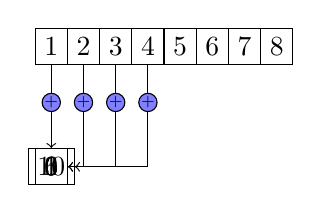
\begin{tikzpicture}[
      start chain=1 going right,start chain=2 going below, node distance=-0.15mm
    ]


  \foreach \x in {1,2,...,8} {
    \node (\x) [draw, on chain=1] {\x};
  }
  
  
  \onslide<2>{
    \node [draw, below=3em of 1] (r1) {0};
  
    }

  
  \onslide<3>{
    \node [draw, below=3em of 1] (r1) {1};
  
    \sumupPrim{1.south}{r1.north}
    }
  
  \onslide<4>{
    \node [draw, below=3em of 1] (r1) {3};
  
    \sumup{2.south}{r1.east}
    }
  
  \onslide<5>{
    \node [draw, below=3em of 1] (r1) {6};
  
    \sumup{3.south}{r1.east}
    }

  \onslide<6>{
    \node [draw, below=3em of 1] (r1) {10};
    \sumup{4.south}{r1.east}
    }




\end{tikzpicture} 
\end{center}
\end{frame}

% -------------------------------------------------------------------------
% Computing a sum in parallel 
% -------------------------------------------------------------------------

\begin{frame}{Data-Parallelism: Sum in Parallel}
\begin{center} 
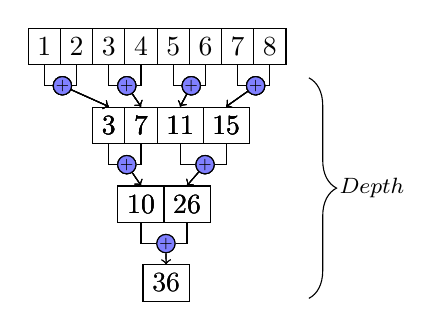
\begin{tikzpicture}[
      start chain=1 going right,start chain=2 going below,node distance=-0.15mm
    ]


  \foreach \x in {1,2,...,8} {
    \node (\x) [draw, on chain=1] {\x};
  }
  
  \onslide<2>{
    \node (imm1) [draw,below=1.5em of 3] {3};
    \node (imm2) [draw,right= of imm1] {7};
    \node (imm3) [draw,right= of imm2] {11};
    \node (imm4) [draw,right= of imm3] {15};
    
    \adder{1}{2}{imm1}
    \adder{3}{4}{imm2}
    \adder{5}{6}{imm3}
    \adder{7}{8}{imm4}
   
  }

  \onslide<3>{
    \node (imm1) [draw,below=1.5em of 3] {3};
    \node (imm2) [draw,right= of imm1] {7};
    \node (imm3) [draw,right= of imm2] {11};
    \node (imm4) [draw,right= of imm3] {15};

    \adder{1}{2}{imm1}
    \adder{3}{4}{imm2}
    \adder{5}{6}{imm3}
    \adder{7}{8}{imm4}
   
    \node (jmm1) [draw,below=1.5em of imm2] {10};
    \node (jmm2) [draw,right= of jmm1] {26};

    \adder{imm1}{imm2}{jmm1}
    \adder{imm3}{imm4}{jmm2} 
  }

 \onslide<4>{
    \node (imm1) [draw,below=1.5em of 3] {3};
    \node (imm2) [draw,right= of imm1] {7};
    \node (imm3) [draw,right= of imm2] {11};
    \node (imm4) [draw,right= of imm3] {15};

    \adder{1}{2}{imm1}
    \adder{3}{4}{imm2}
    \adder{5}{6}{imm3}
    \adder{7}{8}{imm4}

    \node (jmm1) [draw,below=1.5em of imm2] {10};
    \node (jmm2) [draw,right= of jmm1] {26};

    \adder{imm1}{imm2}{jmm1}
    \adder{imm3}{imm4}{jmm2}

    \node (lmm1) [draw,below right=1.5em and -0.8em of jmm1] {36};
    
    \adder{jmm1}{jmm2}{lmm1} 
  }

  %% \onslide<5>{
  %%   \node (imm1) [draw,below=1.5em of 3] {3};
  %%   \node (imm2) [draw,right= of imm1] {7};
  %%   \node (imm3) [draw,right= of imm2] {11};
  %%   \node (imm4) [draw,right= of imm3] {15};

  %%   \adder{1}{2}{imm1}
  %%   \adder{3}{4}{imm2}
  %%   \adder{5}{6}{imm3}
  %%   \adder{7}{8}{imm4}

  %%   \node (jmm1) [draw,below=1.5em of imm2] {10};
  %%   \node (jmm2) [draw,right= of jmm1] {26};

  %%   \adder{imm1}{imm2}{jmm1}
  %%   \adder{imm3}{imm4}{jmm2}

  %%   \node (lmm1) [draw,below right=1.5em and -0.8em of jmm1] {36};
    
  %%   \adder{jmm1}{jmm2}{lmm1}

  %%   \draw [decorate,
  %%          decoration={brace,mirror,amplitude=10pt},xshift=-4pt,yshift=0pt]
  %%         (3.5,-3.2) -- (3.5,-0.4) node [black,midway,xshift=0.8cm]  
  %%         {\footnotesize $Depth$};
  %% }

 \onslide<5>{
    \node (imm1) [draw,below=1.5em of 3] {3};
    \node (imm2) [draw,right= of imm1] {7};
    \node (imm3) [draw,right= of imm2] {11};
    \node (imm4) [draw,right= of imm3] {15};

    \adder{1}{2}{imm1}
    \adder{3}{4}{imm2}
    \adder{5}{6}{imm3}
    \adder{7}{8}{imm4}

    \node (jmm1) [draw,below=1.5em of imm2] {10};
    \node (jmm2) [draw,right= of jmm1] {26};

    \adder{imm1}{imm2}{jmm1}
    \adder{imm3}{imm4}{jmm2}

    \node (lmm1) [draw,below right=1.5em and -0.8em of jmm1] {36};
    
    \adder{jmm1}{jmm2}{lmm1}

    \draw [decorate,
           decoration={brace,mirror,amplitude=10pt},xshift=-4pt,yshift=0pt]
          (3.5,-3.2) -- (3.5,-0.4) node [black,midway,xshift=0.8cm]  
          {\footnotesize $Depth$};
         
  }
\end{tikzpicture} 

\onslide<5>{
   \begin{tikzpicture}[overlay,remember picture] 
      
    \node [fill=red!50,single arrow] at (-3.7,3.5) {\tiny Potential for parallelism};
    \node [fill=red!50,single arrow] at (-2.8,2.4) {\tiny Potential for parallelism};
    \end{tikzpicture}
 
}


\end{center}
\end{frame}

% -------------------------------------------------------------------------
%
% -------------------------------------------------------------------------

\begin{frame}{Data-Parallelism}

  \begin{columns} 

  \begin{column}{.48\textwidth}
  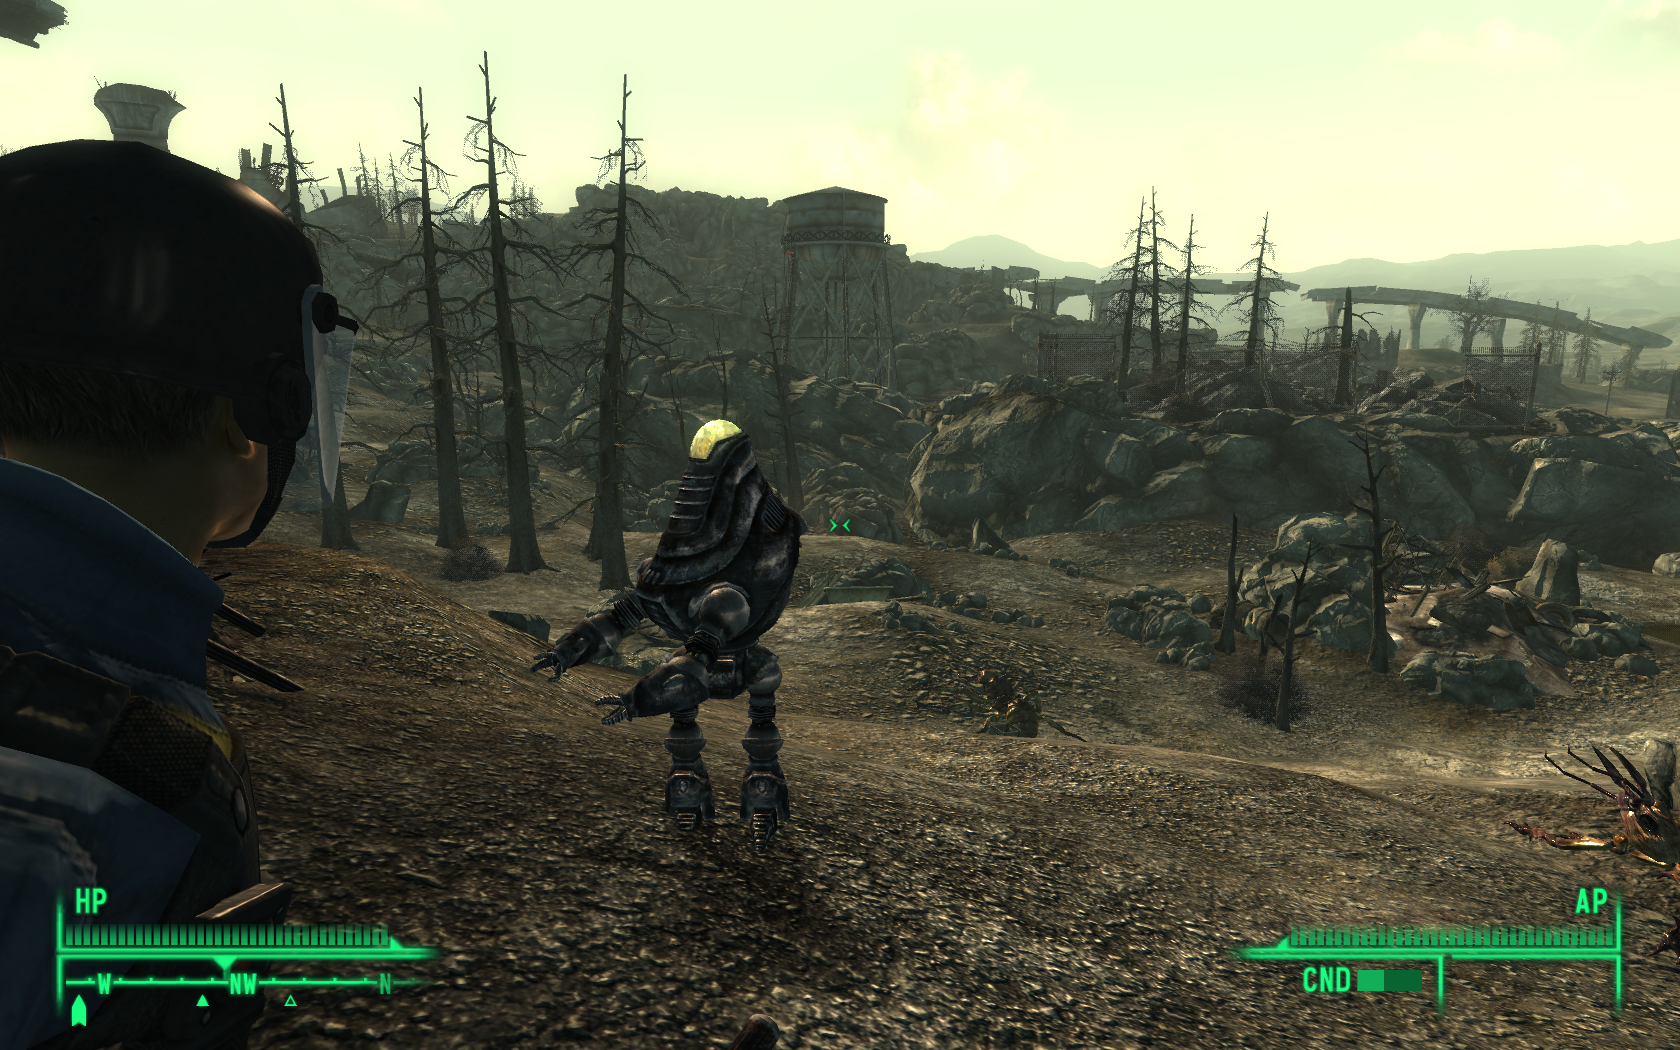
\includegraphics[width=\linewidth]{fallout.jpg}

  Rendering

  \vspace{1cm}
  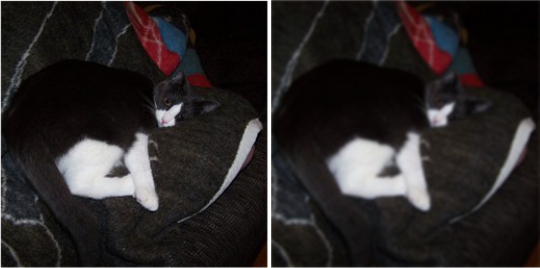
\includegraphics[width=\linewidth]{kiri.jpg}

  Image processing

  \end{column} 
  
  \begin{column}{.48\textwidth} 
  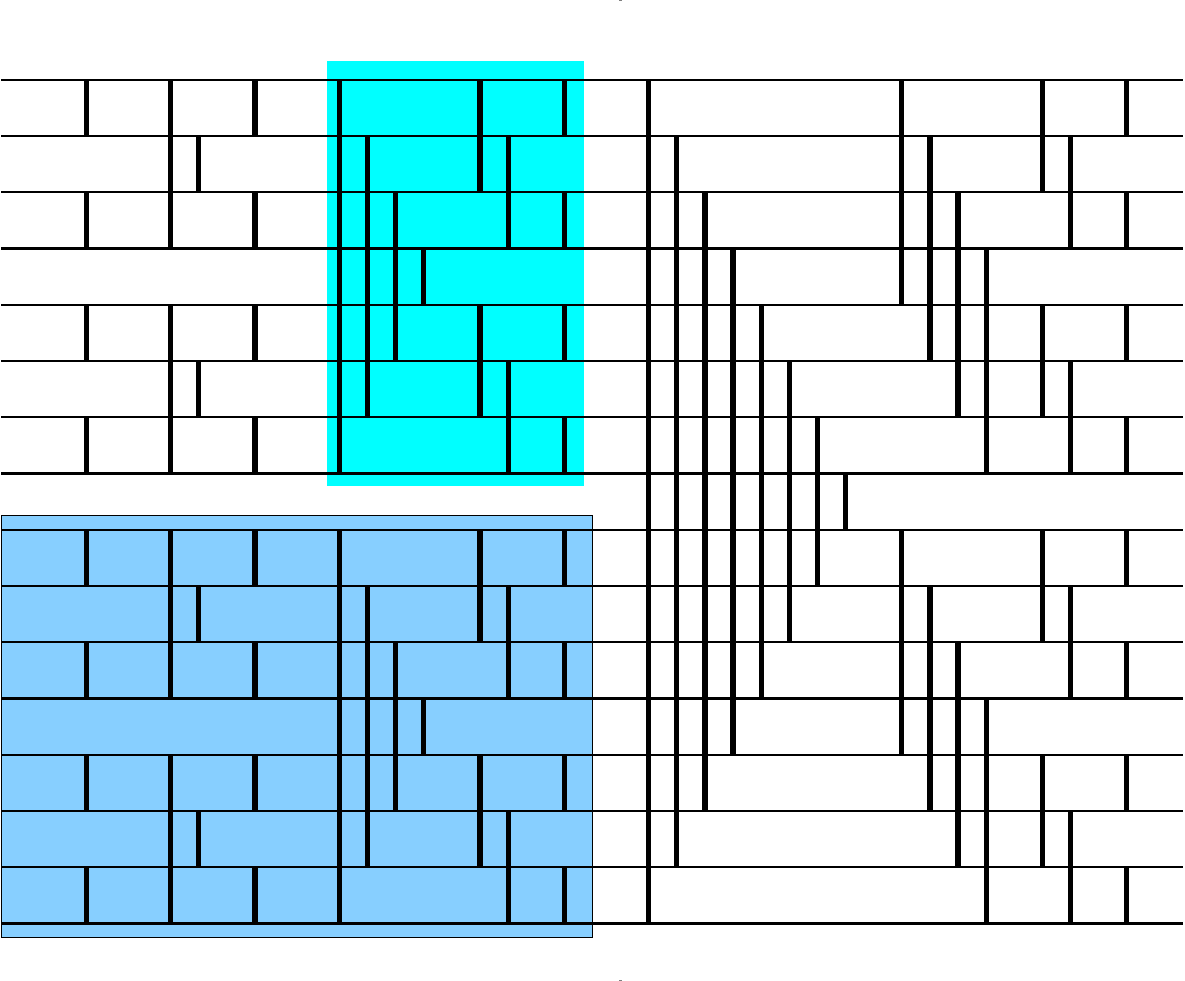
\includegraphics[width=\linewidth]{mmixedsorter.pdf}

  Sorting

  \end{column}
  
  \end{columns}

\end{frame}


\begin{frame}{Data-Parallelism}

  \begin{itemize} 
    \item Scalable
      \begin{itemize} 
        \item Potential for parallelism increases with data size 
      \end{itemize}
    \item Fine grained parallelism 
  \end{itemize} 

\end{frame}

% -------------------------------------------------------------------------
%
% -------------------------------------------------------------------------
\section{GPUs and CUDA}

\begin{frame}{GPUs} 
  \begin{center}
  {\Large Graphics Processing Units}
  \end{center}
\end{frame} 


\begin{frame}{GPUs} 

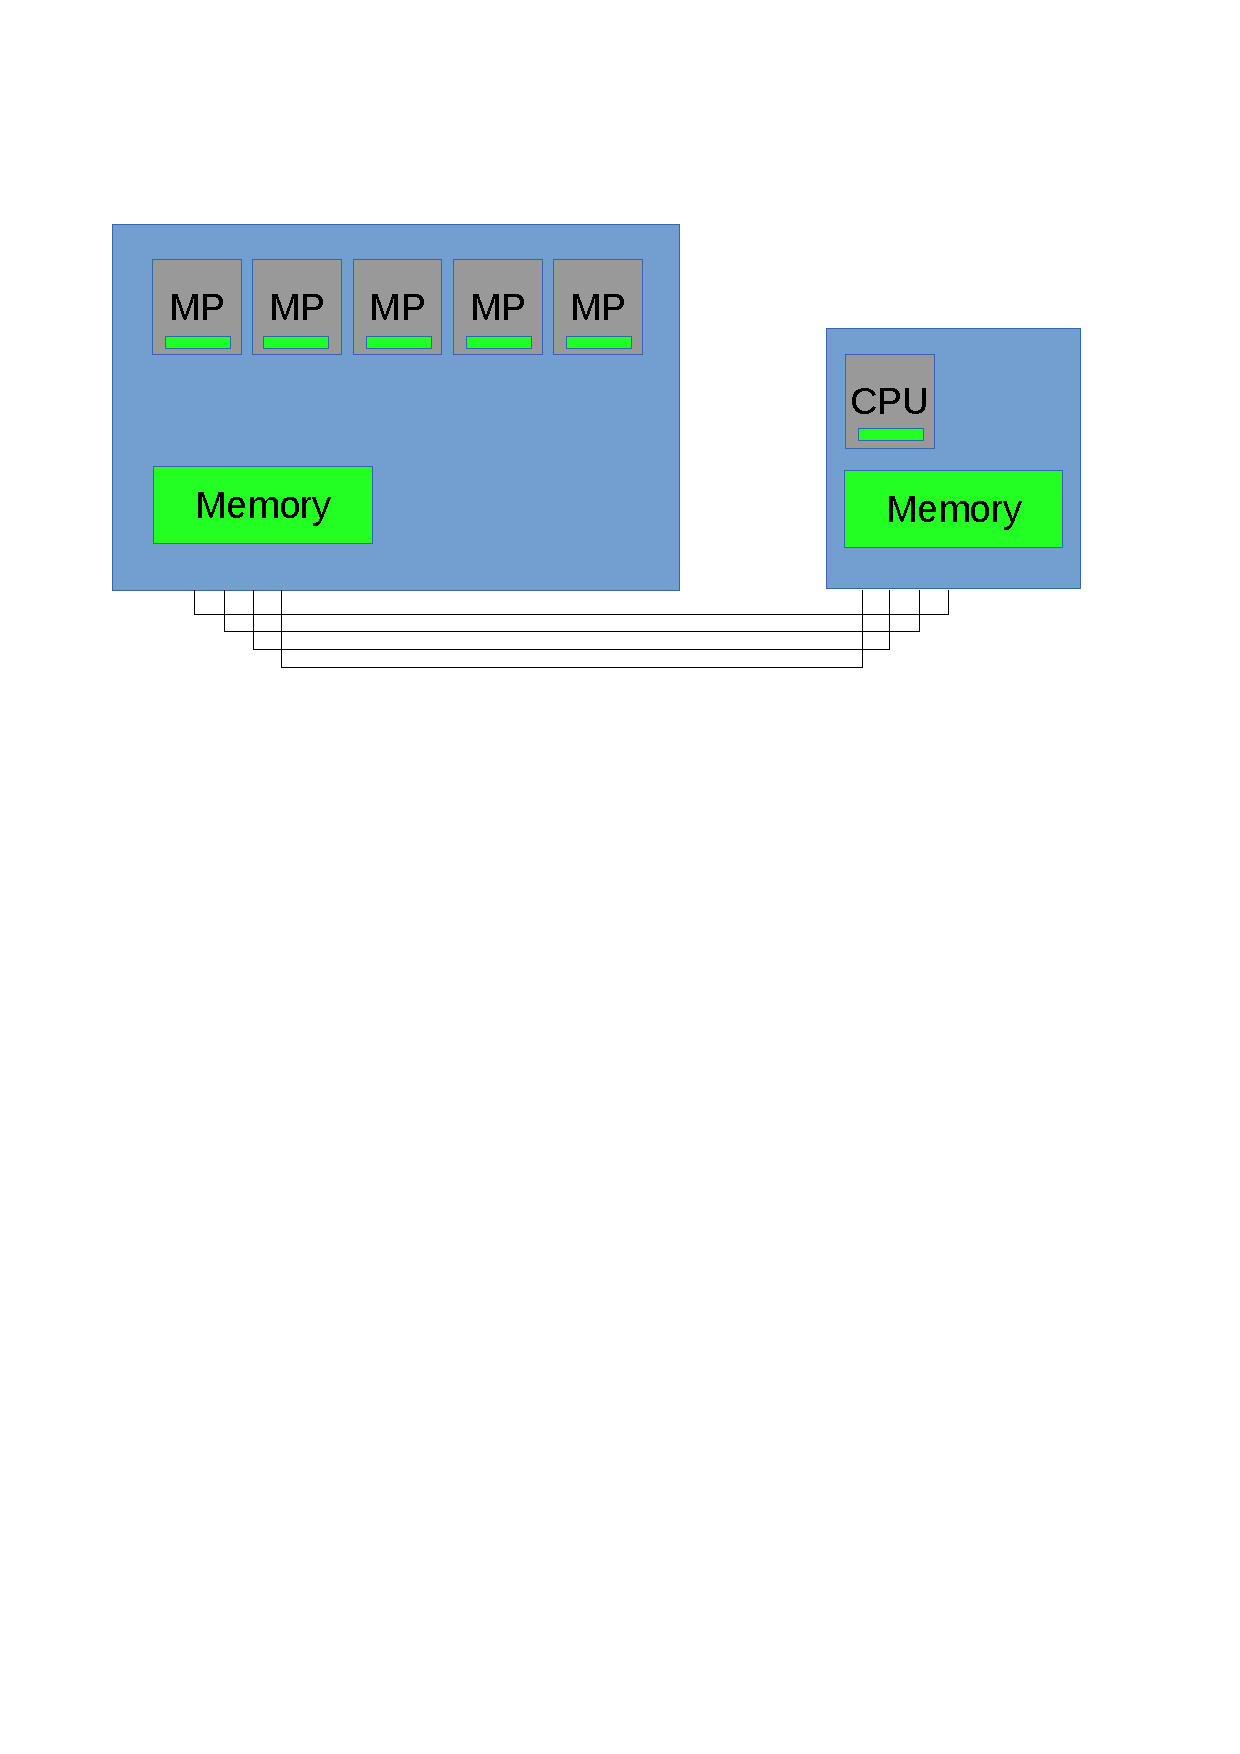
\includegraphics[width=\linewidth]{GPU1.pdf}


\end{frame} 

\begin{frame}{GPUs} 

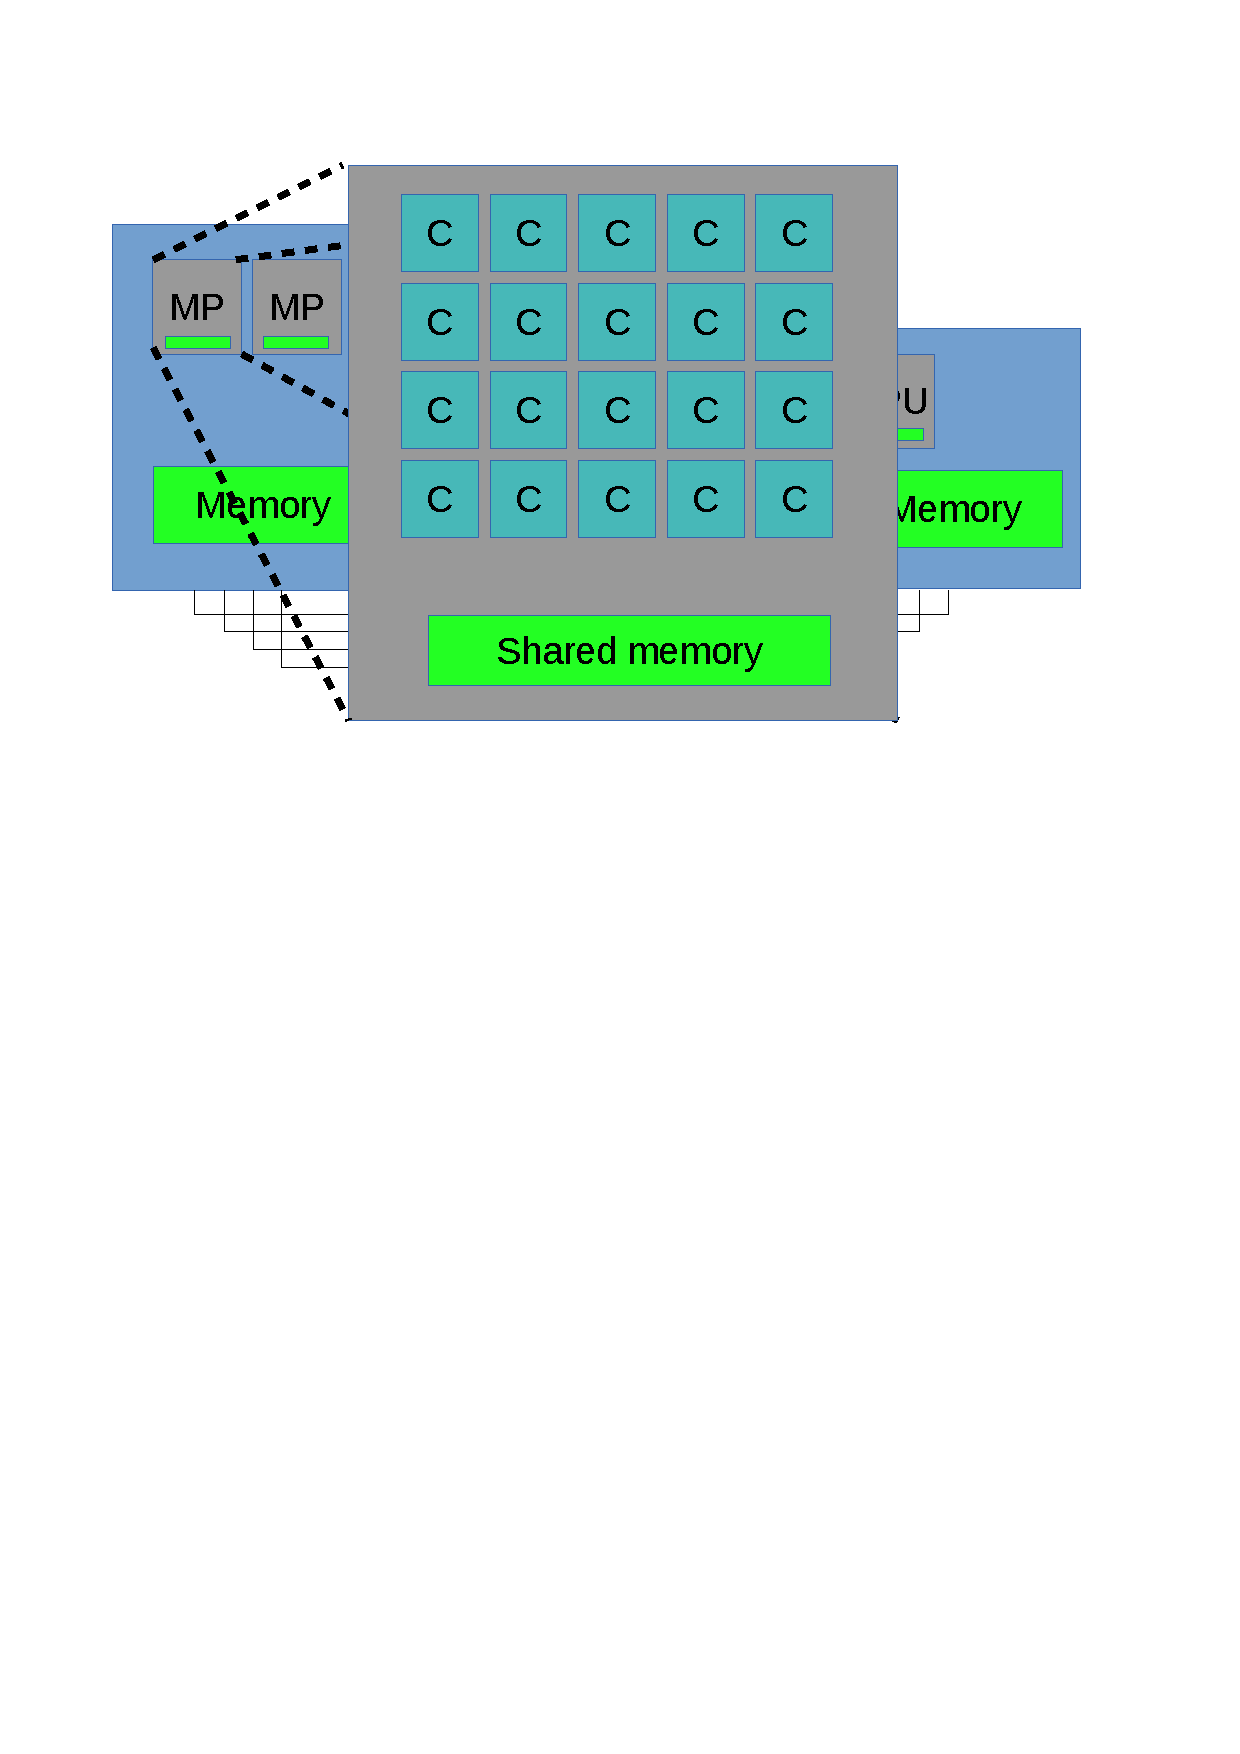
\includegraphics[width=\linewidth]{GPU2.pdf}


\end{frame} 


% -------------------------------------------------------------------------
%
% -------------------------------------------------------------------------

\begin{frame}{GPU Programming: CUDA Terminology} 
  
  \begin{itemize} 
    \item Thread:
      \begin{itemize} 
        \item Sequential work
        \item Executed on a core
      \end{itemize}
    \item Warp:
      \begin{itemize} 
        \item 32 threads
        \item Scheduled unit
        \item Lockstep
      \end{itemize}
    \item Block: 
      \begin{itemize} 
        \item Up 1024 threads 
        \item Executes on the MPs
        \item Shared memory 
        \item Thread synchronisation
      \end{itemize} 
    \item Grid: Collection of all blocks
  \end{itemize} 

\end{frame}


% -------------------------------------------------------------------------
%
% -------------------------------------------------------------------------
\begin{frame}[fragile]{GPU Programming: CUDA Example}

\begin{block}{}
\begin{verbatim} 
__global__ void inc(int32_t *a, int32_t *r) {
  
  unsigned int gid = blockIdx.x * 
                     blockDim.x + 
                     threadIdx.x;

  r[gid] = a[gid] + 1; 

} 
\end{verbatim}
\end{block} 


\end{frame} 

% -------------------------------------------------------------------------
%
% -------------------------------------------------------------------------

\begin{frame}{GPU Programming} 

  Things to consider:

  \begin{itemize} 
    \item Minimise data transfer between host and device
    \item Coalesce global memory accesses
    \item Minimise use of global memory 
   % \item Avoid different execution paths within a block
   % \item Be careful with {\tt \_\_syncthreads} and conditionals
  \end{itemize} 
  
\end{frame} 


% -------------------------------------------------------------------------
%
% -------------------------------------------------------------------------
\section{Embedded Languages: Background}


\begin{frame}{Embedded Languages} 
 \begin{center}
   {\Large Embedded Languages}
 \end{center}
%%
%%  Embedding ArBB, similar slides to Obsidian, more pictures. 

\end{frame} 


\begin{frame}[fragile]{Embedded Languages: Background} 
  
  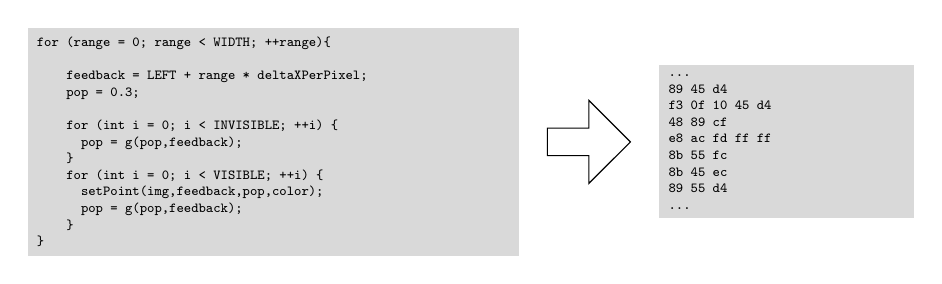
\begin{tikzpicture} 

    \node [fill=gray!30] (cuda) {
      \begin{minipage}{6cm}
        \begin{tiny} 
\begin{verbatim}
for (range = 0; range < WIDTH; ++range){

    feedback = LEFT + range * deltaXPerPixel;
    pop = 0.3;

    for (int i = 0; i < INVISIBLE; ++i) {
      pop = g(pop,feedback);
    }
    for (int i = 0; i < VISIBLE; ++i) {
      setPoint(img,feedback,pop,color);
      pop = g(pop,feedback);
    }
}
\end{verbatim}    
\end{tiny}    
\end{minipage}
};
    \node [draw,single arrow,right=1em of cuda, minimum size=3em] (arr) {};
    
    \node [fill=gray!30,right=1em of arr] (mc) { 
      \begin{minipage}{3cm}
\begin{tiny}
\begin{verbatim}
...
89 45 d4             
f3 0f 10 45 d4
48 89 cf
e8 ac fd ff ff
8b 55 fc      
8b 45 ec      
89 55 d4      
...
\end{verbatim}
\end{tiny}
      \end{minipage}
    };
      
      
    
  \end{tikzpicture}

  
\end{frame} 

% -------------------------------------------------------------------------
%
% -------------------------------------------------------------------------

% -------------------------------------------------------------------------
%
% -------------------------------------------------------------------------
\begin{frame}[fragile]{Embedded Languages: {\small Embedded Four-Function Calculator}}

\begin{block}{}
\begin{verbatim} 
import Prelude hiding (div) 
import qualified Prelude as P

data Op = Add | Sub | Mul | Div 

data Expr = Bin Expr Op Expr | Lit Int 

eval (Bin e1 op e2) =
  let (e1', e2') = (eval e1, eval e2) in
    case op of Add -> e1' + e2'
               Sub -> e1' - e2'
               Mul -> e1' * e2'
               Div -> e1' `P.div` e2'

eval (Lit i) = i
\end{verbatim}  
\end{block} 

\end{frame} 

% -------------------------------------------------------------------------
%
% -------------------------------------------------------------------------
\begin{frame}[fragile]{Embedded Languages: {\small Embedded Four-Function Calculator}} 

\begin{block}{}
\begin{verbatim} 
instance Num Expr where
  (+) a b = Bin a Add b 
  (-) a b = Bin a Sub b
  (*) a b = Bin a Mul b 
  fromInteger = Lit . fromInteger

div a b = Bin a Div b 
\end{verbatim}  
\end{block} 

\end{frame} 

% -------------------------------------------------------------------------
%
% -------------------------------------------------------------------------
\begin{frame}[fragile]{Embedded Languages: {\small Embedded Four-Function Calculator}} 

\begin{block}{}
\begin{verbatim} 
ex1 :: Expr
ex1 = 9*1+2
\end{verbatim}  
\end{block} 

\pause
\begin{block}{}
\begin{verbatim} 
ex2 :: Expr -> Expr
ex2 x = a+a 
  where
    a = x*x
\end{verbatim}  
\end{block} 

\pause
\begin{block}{}
\begin{verbatim} 
ex3 :: Expr
ex3 = P.sum (map fromInteger [0..15])
\end{verbatim}  
\end{block} 

\end{frame} 


% -------------------------------------------------------------------------
%
% -------------------------------------------------------------------------
\section{Obsidian}

% -------------------------------------------------------------------------
%
% -------------------------------------------------------------------------



\begin{frame}{Obsidian} 
  
  \begin{center}
  {\Large Embedded Language for GPU Kernel Implementation}
  \end{center}
  %% \begin{itemize} 
  %%   \item Our level of GPU programming 
  %%   \item Programming example  (reduction) 
  %%   \item Performance 
  %%   \item Compare to related approaches 
  %% \end{itemize}
      
\end{frame} 

% -------------------------------------------------------------------------
%
% -------------------------------------------------------------------------

\begin{frame}{Obsidian} 
  Obsidian: 
  \begin{itemize} 
    \item Embedded in Haskell
    \item Encourage experimentation
    \item Higher level than CUDA 
      \begin{itemize} 
        \item Not as much indexing magic
        \item Programs describe ``whole'' computation
        \item Code reuse 
        \item Still have control over low level details
      \end{itemize} 
  \end{itemize}  
\end{frame}

\begin{frame}[fragile]{Obsidian: Arrays}
  
  Pull and Push arrays: 
  \begin{itemize}
  \item Represents ways to compute arrays, \\
        not data in memory
  \item Operations on them fuse by default \newline
    \verb!map f . map g!
  \item Programmer can choose not to fuse
    \begin{itemize} 
    \item by inserting a {\tt force} operation
    \end{itemize}
  \item Parallel
  \end{itemize} 
     
\end{frame} 


\begin{frame}{Obsidian} 

\begin{center}
\def\s{.50}

\tikzstyle{mybox} = [draw=black, fill=blue!20, very thick,
    rectangle, rounded corners, inner sep=10pt, inner ysep=20pt]

\tikzstyle{wbox} = [draw=black, very thick,
    rectangle, rounded corners, inner sep=10pt, inner ysep=20pt]

\tikzstyle{smallbox} = [draw=black, fill=green!20, very thick,
    rectangle, rounded corners, inner sep=10pt, inner ysep=7pt]

\tikzstyle{fancytitle} =[fill=red, text=white]

\begin{tikzpicture}[scale=(\s)]

%\draw [help lines] (0,0) grid (16,10);

\node [mybox] (Grid){%
    \begin{minipage}{0.15\linewidth}
        Grid
    \end{minipage}
};
\node [mybox,below=0cm of Grid.south] (Block){%
    \begin{minipage}{0.15\linewidth}
        Block
    \end{minipage}
};
\node [mybox,below=0cm of Block.south] (Thread){%
    \begin{minipage}{0.15\linewidth}
        Thread
    \end{minipage}
};

\node [smallbox,right=0cm of Grid.north east, anchor=north west] (gd) {%
    \begin{minipage}{0.25\linewidth}
        {\small Global memory}
    \end{minipage}
};

\node [smallbox,right=0cm of Block.north east, anchor=north west] (bd) {%
    \begin{minipage}{0.25\linewidth}
        {\small Shared memory}
    \end{minipage}
};

\node [smallbox,right=0cm of Block.south east, anchor=south west] (sync) {%
    \begin{minipage}{0.25\linewidth}
        {\small Syncthreads}
    \end{minipage}
};

\node [smallbox,right=0cm of Thread.north east, anchor=north west] (td) {%
    \begin{minipage}{0.25\linewidth}
        {\small Reg to reg}
    \end{minipage}
};

\node [smallbox, right=0cm of Thread.south east, anchor=south west] (seq) {%
    \begin{minipage}{0.25\linewidth}
        {\small Sequential}
    \end{minipage}
};

\node [below=2mm of Thread] (l1) {\small Level};
\node [right=11mm of l1.north east, anchor=north west] (l2) {\small Key concepts};
\node [right=16mm of l2.north east, anchor=north west] (l3) {\small Obsidian};

\node [wbox,inner ysep=13pt,right=0cm of gd.north east, anchor=north west] (obs1) {% 
  \begin{minipage}{0.35\linewidth}
        {\small pConcat, generate, \\DPush, DPull}
    \end{minipage}
};

\node [wbox,inner ysep=13pt,below=0cm of obs1.south] (obs2) {% 
  \begin{minipage}{0.35\linewidth}
        {\small pConcat, generate, force, SPush, SPull}
    \end{minipage}
};

\node [wbox,inner ysep=5.5pt, below=0cm of obs2.south] (obs3) {% 
  \begin{minipage}{0.35\linewidth}
        {\small seqFor, seqUntil \\ seqReduce\\ seqScan, SPush, SPull}
    \end{minipage}
};

\end{tikzpicture}

%% \onslide<2>{ 
%%   \begin{tikzpicture}[overlay, remember picture]
    
%%     \node [draw, fill=red!50,minimum width = 6em, thick, rounded corners] at (-4,3) {Warp};
    
%%   \end{tikzpicture}


%% } 
\end{center}
\end{frame}


% -------------------------------------------------------------------------
%
% -------------------------------------------------------------------------

\begin{frame}[fragile]{Obsidian: Simple Example}

\begin{block}{} 
\begin{verbatim} 
inc :: Num a => SPull a -> SPull a
inc = fmap (+1)
\end{verbatim} 
\end{block} 

\pause 
\begin{block}{} 
\begin{verbatim} 
incK :: Num a => DPull (SPull a) -> DPush Grid a
incK = pConcatMap (push . inc)
\end{verbatim} 
\end{block} 


\end{frame} 

% -------------------------------------------------------------------------
%
% -------------------------------------------------------------------------
\newcommand\Fontvi{\fontsize{8}{7.2}\selectfont}

\begin{frame}[fragile]{Obsidian: Generated Code}
\begin{block}{256 threads and 256 elements per block} 
\Fontvi
\begin{verbatim} 
extern "C" __global__ void inc(int32_t* input0, uint32_t n0,
                               int32_t* output1)
{
    uint32_t tid = threadIdx.x;
     
    if (blockIdx.x < n0 / 256U) {
        output1[blockIdx.x * 256U + tid] = 
          input0[blockIdx.x * 256U + tid] + 1;
    }
}
\end{verbatim} 

\end{block}
\end{frame}

% -------------------------------------------------------------------------
%
% -------------------------------------------------------------------------
\begin{frame}[fragile]{Obsidian: Generated Code}
\begin{block}{128 threads and 256 elements per block}
\Fontvi
\begin{verbatim} 
extern "C" __global__ void inc(int32_t* input0, uint32_t n0,
                               int32_t* output1)
{
    uint32_t tid = threadIdx.x;
    
    if (blockIdx.x < n0 / 256U) {
        for (int i = 0; i < 2; ++i) {
            tid = i * 128 + threadIdx.x;
            output1[blockIdx.x * 256U + tid] = 
              input0[blockIdx.x * 256U + tid] + 1;
        }
        tid = threadIdx.x;
    }
}
\end{verbatim} 
\end{block} 


\end{frame} 

% ---------------------------------------------------------------------------
%
% ---------------------------------------------------------------------------

\begin{frame}{Obsidian: Reduction Experimentation}

  
% Figures that illustrate optimisation effort of Reduction kernels 

%% \newcommand{\arrayLength}[1]{%
%%   \setcounter{arraycard}{0}%
%%   \foreach \x in #1{%
%%     \stepcounter{arraycard}%
%%   }%
%%   \the\value{arraycard}%
%% }  

% smrow{x}{y}{data}{largest_index}{identifier}
\newcommand{\smRow}[5] { 
  
 %                                       (INSANE!) 
  \node [draw, fill=gray!30,anchor=west] (#50) at (#1,#2) {\pgfmathparse{#3[0]}\pgfmathresult};   
  
  \ifnum#4>0
    \foreach[count=\i] \j in {1,...,#4} {
      \pgfmathtruncatemacro{\n}{int(\i) - 1};
      \pgfmathtruncatemacro{\m}{int(\i)};
      \node [draw, fill=gray!30,right=0cm of #5\n,anchor=west] (#5\m) {\pgfmathparse{#3[\j]}\pgfmathresult};   % {\j};   
    } 
  \fi
}


% smRowTiny{x}{y}{data}{largest_index}{identifier} 
\newcommand{\smRowTiny}[5] { 
  
 %                                       
  \node [draw, fill=gray!30,anchor=west,inner sep=1pt] (#50) at (#1,#2) {\tiny\pgfmathparse{#3[0]}\pgfmathresult};   
  
  \ifnum#4>0
    \foreach[count=\i] \j in {1,...,#4} {
      \pgfmathtruncatemacro{\n}{int(\i) - 1};
      \pgfmathtruncatemacro{\m}{int(\i)};
      \node [draw, fill=gray!30,right=0cm of #5\n,anchor=west,inner sep=1pt] (#5\m) {\tiny\pgfmathparse{#3[\j]}\pgfmathresult};   % {\j};   
    } 
  \fi
}

\newcommand{\seqRed}[3] { 
 \tikzset{sstyle/.style={anchor=west,draw,shape=circle,fill,inner sep=1pt}};
 \tikzset{cstyle/.style={anchor=west,draw,shape=circle,inner sep=0pt}};
 %\tikzstyle{every node}=[anchor=west,draw,shape=circle,fill,inner sep=1pt]

 \node [sstyle](r1) at (0+ #1,#2) {};
 \node [sstyle,right=.5mm of r1] (r2) {};
 \node [sstyle,right=.5mm of r2] (r3) {};
 \node [sstyle,right=.5mm of r3] (r4) {};

 
 \path [draw] (r1) -- (r2) ;
 \path [draw] (r2) -- (r3) ;
 \path [draw] (r3) -- (r4) ;
 
 % connectors 

 %\tikzstyle{every node}=[anchor=west,draw,shape=circle,inner sep=0pt]

 \node [cstyle,above=.5mm of r1] (#3c1) {};
 \node [cstyle,above=.5mm of r2] (#3c2) {};
 \node [cstyle,above=.5mm of r3] (#3c3) {};
 \node [cstyle,above=.5mm of r4] (#3c4) {};

 \node [cstyle,below=.5mm of r4] (#3c5) {};

 % wires 

 \path [draw] (r1) -- (#3c1) ;
 \path [draw] (r2) -- (#3c2) ;
 \path [draw] (r3) -- (#3c3) ;
 \path [draw] (r4) -- (#3c4) ;
 \path [draw] (r4) -- (#3c5) ;


}



%\foreach[count=\i] \j in {1,1,1,1,1,1,1,1} { 
%  \pgfmathtruncatemacro{\n}{int(\i)};
%  \node[draw=black] (a\n) at (\i,-2) {\j};
%}



\begin{figure} 

% --------------------------------------------------------------------------- 
% Pair fmap 
% ---------------------------------------------------------------------------
\begin{minipage}{.45\linewidth} 
\begin{tikzpicture}[scale = 0.40]

\smRow{0}{0}{{0,1,2,3,4,5,6,7}}{7}{a}

\smRow{0}{-2}{{1,5,9,13}}{3}{b}

\smRow{0}{-4}{{6,22}}{1}{c}

\smRow{0}{-6}{{28,0}}{0}{d}  % HACK

%% \smRow{0}{0}{{0,1,2,3,4,5,6,7}}{7}{a}

%% \smRow{1.75}{-2}{{1,5,9,13}}{3}{b}

%% \smRow{2.5}{-4}{{6,22}}{1}{c}

%% \smRow{3}{-6}{{28,0}}{0}{d}  % HACK

% connections 


\path[->,draw=black] (a0.south) -- (b0.north) ; 
\path[->,draw=black] (a1.south) -- (b0.north) ; 

\path[->,draw=black] (a2.south) -- (b1.north) ; 
\path[->,draw=black] (a3.south) -- (b1.north) ; 

\path[->,draw=black] (a4.south) -- (b2.north) ; 
\path[->,draw=black] (a5.south) -- (b2.north) ; 

\path[->,draw=black] (a6.south) -- (b3.north) ; 
\path[->,draw=black] (a7.south) -- (b3.north) ; 


\path[->,draw=black] (b0.south) -- (c0.north) ; 
\path[->,draw=black] (b1.south) -- (c0.north) ; 

\path[->,draw=black] (b2.south) -- (c1.north) ; 
\path[->,draw=black] (b3.south) -- (c1.north) ; 

\path[->,draw=black] (c0.south) -- (d0.north) ; 
\path[->,draw=black] (c1.south) -- (d0.north) ; 


\end{tikzpicture} 

\end{minipage}
\hfill%hspace{2mm}%
% --------------------------------------------------------------------------- 
% Halve zip  
% ---------------------------------------------------------------------------
\begin{minipage}{.45\linewidth} 
\begin{tikzpicture}[scale = 0.40]

\smRow{0}{0}{{0,1,2,3,4,5,6,7}}{7}{a}

\smRow{0}{-2}{{4,6,8,10}}{3}{b}

\smRow{0}{-4}{{12,16}}{1}{c}

\smRow{0}{-6}{{28,0}}{0}{d}  % HACK

%% \smRow{0}{0}{{0,1,2,3,4,5,6,7}}{7}{a}

%% \smRow{1.75}{-2}{{4,6,8,10}}{3}{b}

%% \smRow{2.5}{-4}{{12,16}}{1}{c}

%% \smRow{3.25}{-6}{{28,0}}{0}{d}  % HACK

% connections 


\path[->,draw=black] (a0.south) -- (b0.north) ; 
\path[->,draw=black] (a4.south) -- (b0.north) ; 

\path[->,draw=black] (a1.south) -- (b1.north) ; 
\path[->,draw=black] (a5.south) -- (b1.north) ; 

\path[->,draw=black] (a2.south) -- (b2.north) ; 
\path[->,draw=black] (a6.south) -- (b2.north) ; 

\path[->,draw=black] (a3.south) -- (b3.north) ; 
\path[->,draw=black] (a7.south) -- (b3.north) ; 


\path[->,draw=black] (b0.south) -- (c0.north) ; 
\path[->,draw=black] (b2.south) -- (c0.north) ; 

\path[->,draw=black] (b1.south) -- (c1.north) ; 
\path[->,draw=black] (b3.south) -- (c1.north) ; 

\path[->,draw=black] (c0.south) -- (d0.north) ; 
\path[->,draw=black] (c1.south) -- (d0.north) ; 



\end{tikzpicture} 

\end{minipage}

%% \caption{\emph{Left:} {\tt evenOdds} - {\tt zipWith} reduction, leads to uncoalesced memory accesses.\newline
%% \emph{Right:} {\tt halve} - {\tt zipWith} reduction, leads to coalesced memory accesses.
%% This coalescing is most important during the very first phase, when data is 
%% read from global memory.} 

\label{fig:red1}
\end{figure} 



% ---------------------------------------------------------------------------
% Sequential reductions 
% ---------------------------------------------------------------------------


%% \begin{figure} 

%% \begin{tikzpicture}[scale = 0.40]

%% \smRowTiny{0}{{0,1,2,3,4,5,6,7,8,9,10,11,12,13,14,15,16,17,18,19,20,21,22,23,24,25,26,27,28,29,30,31}}{31}{a}

%% \seqRed{0}{-2}{redA}
%% \seqRed{2}{-2}{redB}
%% \seqRed{4}{-2}{redC}
%% \seqRed{6}{-2}{redD}
%% \seqRed{8}{-2}{redE}
%% \seqRed{10}{-2}{redF}
%% \seqRed{12}{-2}{redG}
%% \seqRed{14}{-2}{redH}

%% % connections 
%% \foreach[count=\i] \j in {redAc1,redAc2,redAc3,redAc4, 
%%                           redBc1,redBc2,redBc3,redBc4, 
%%                           redCc1,redCc2,redCc3,redCc4, 
%%                           redDc1,redDc2,redDc3,redDc4, 
%%                           redEc1,redEc2,redEc3,redEc4, 
%%                           redFc1,redFc2,redFc3,redFc4, 
%%                           redGc1,redGc2,redGc3,redGc4, 
%%                           redHc1,redHc2,redHc3,redHc4} {
%%   \pgfmathtruncatemacro{\n}{int(\i) - 1};
%%   \path[draw=black] (a\n.south) -- (\j.north) ; 
%% %\path[draw=black] (a1.south) -- (redAc2.north) ; 
%% %\path[draw=black] (a2.south) -- (redAc3.north) ; 
%% %\path[draw=black] (a3.south) -- (redAc4.north) ; 
%% } 

%% %next row of sM

%% \smRowTiny{-4}{{6,22,38,54,70,86,102,118}}{7}{b}

%% %connections 

%% \path[draw=black] (redAc5) -- (b0.north); 
%% \path[draw=black] (redBc5) -- (b1.north); 
%% \path[draw=black] (redCc5) -- (b2.north); 
%% \path[draw=black] (redDc5) -- (b3.north); 
%% \path[draw=black] (redEc5) -- (b4.north); 
%% \path[draw=black] (redFc5) -- (b5.north); 
%% \path[draw=black] (redGc5) -- (b6.north); 
%% \path[draw=black] (redHc5) -- (b7.north); 



%% %% \path[->,draw=black] (a0.south) -- (b0.north) ; 
%% %% \path[->,draw=black] (a1.south) -- (b0.north) ; 

%% %% \path[->,draw=black] (a2.south) -- (b1.north) ; 
%% %% \path[->,draw=black] (a3.south) -- (b1.north) ; 

%% %% \path[->,draw=black] (a4.south) -- (b2.north) ; 
%% %% \path[->,draw=black] (a5.south) -- (b2.north) ; 

%% %% \path[->,draw=black] (a6.south) -- (b3.north) ; 
%% %% \path[->,draw=black] (a7.south) -- (b3.north) ; 


%% %% \path[->,draw=black] (b0.south) -- (c0.north) ; 
%% %% \path[->,draw=black] (b1.south) -- (c0.north) ; 

%% %% \path[->,draw=black] (b2.south) -- (c1.north) ; 
%% %% \path[->,draw=black] (b3.south) -- (c1.north) ; 

%% %% \path[->,draw=black] (c0.south) -- (d0.north) ; 
%% %% \path[->,draw=black] (c1.south) -- (d0.north) ; 


%% \end{tikzpicture} 


%% \caption{Adding sequential reductions like this, reintroduces memory coalescing issues. 
%%  Consecutive threads nolonger access consecutive memory locations.} 

%% \label{fig:red1}
%% \end{figure} 




%% %%%%%%%%%%%%%%%%%%%%%%%%%%%%%%%%%%%%%%%%%%%%%%%%%%%%%%%%%%%%%%%%%%%%%%%%%%%
%%
%%  REINTRODUCE COALESCING
%%
%% %%%%%%%%%%%%%%%%%%%%%%%%%%%%%%%%%%%%%%%%%%%%%%%%%%%%%%%%%%%%%%%%%%%%%%%%%%%



\begin{figure} 

\begin{minipage}{0.45\linewidth}
\begin{tikzpicture}[scale = 0.40]

%\smRowTiny{0}{{0,1,2,3,4,5,6,7,8,9,10,11,12,13,14,15,16,17,18,19,20,21,22,23,24,25,26,27,28,29,30,31}}{31}{a}
\smRowTiny{0}{0}{{0,1,2,3,4,5,6,7,8,9,10,11,12,13,14,15}}{15}{a}

\seqRed{0}{-2}{redA}
\seqRed{2}{-2}{redB}
\seqRed{4}{-2}{redC}
\seqRed{6}{-2}{redD}
%\seqRed{8}{-2}{redE}
%\seqRed{10}{-2}{redF}
%\seqRed{12}{-2}{redG}
%\seqRed{14}{-2}{redH}

% connections 
\foreach[count=\i] \j in {redAc1,redAc2,redAc3,redAc4, 
                          redBc1,redBc2,redBc3,redBc4, 
                          redCc1,redCc2,redCc3,redCc4, 
                          redDc1,redDc2,redDc3,redDc4} {
                         
  \pgfmathtruncatemacro{\n}{int(\i) - 1};
  \path[draw=black] (a\n.south) -- (\j.north) ; 
} 

%next row of sM

%\smRowTiny{-4}{{6,22,38,54,70,86,102,118}}{7}{b}
\smRowTiny{0}{-4}{{6,22,38,54}}{3}{b}
%\smRowTiny{3}{-4}{{6,22,38,54}}{3}{b}


%connections 

\path[draw=black] (redAc5) -- (b0.north); 
\path[draw=black] (redBc5) -- (b1.north); 
\path[draw=black] (redCc5) -- (b2.north); 
\path[draw=black] (redDc5) -- (b3.north); 
%\path[draw=black] (redEc5) -- (b4.north); 
%\path[draw=black] (redFc5) -- (b5.north); 
%\path[draw=black] (redGc5) -- (b6.north); 
%\path[draw=black] (redHc5) -- (b7.north); 



%% \path[->,draw=black] (a0.south) -- (b0.north) ; 
%% \path[->,draw=black] (a1.south) -- (b0.north) ; 

%% \path[->,draw=black] (a2.south) -- (b1.north) ; 
%% \path[->,draw=black] (a3.south) -- (b1.north) ; 

%% \path[->,draw=black] (a4.south) -- (b2.north) ; 
%% \path[->,draw=black] (a5.south) -- (b2.north) ; 

%% \path[->,draw=black] (a6.south) -- (b3.north) ; 
%% \path[->,draw=black] (a7.south) -- (b3.north) ; 


%% \path[->,draw=black] (b0.south) -- (c0.north) ; 
%% \path[->,draw=black] (b1.south) -- (c0.north) ; 

%% \path[->,draw=black] (b2.south) -- (c1.north) ; 
%% \path[->,draw=black] (b3.south) -- (c1.north) ; 

%% \path[->,draw=black] (c0.south) -- (d0.north) ; 
%% \path[->,draw=black] (c1.south) -- (d0.north) ; 


\end{tikzpicture} 

%\label{fig:red1}

%\end{figure} 
\end{minipage}\hfill%\hspace{2mm}%
\begin{minipage}{0.45\linewidth}
%\begin{figure} 
%
\begin{tikzpicture}[scale = 0.40]

%\smRowTiny{0}{{0,1,2,3,4,5,6,7,8,9,10,11,12,13,14,15,16,17,18,19,20,21,22,23,24,25,26,27,28,29,30,31}}{31}{a}
\smRowTiny{0}{0}{{0,1,2,3,4,5,6,7,8,9,10,11,12,13,14,15}}{15}{a}

\seqRed{0}{-2}{redA}
\seqRed{2}{-2}{redB}
\seqRed{4}{-2}{redC}
\seqRed{6}{-2}{redD}
%\seqRed{8}{-2}{redE}
%\seqRed{10}{-2}{redF}
%\seqRed{12}{-2}{redG}
%\seqRed{14}{-2}{redH}

% connections 
\foreach[count=\i] \j in {redAc1,redBc1,redCc1,redDc1, 
                          redAc2,redBc2,redCc2,redDc2, 
                          redAc3,redBc3,redCc3,redDc3, 
                          redAc4,redBc4,redCc4,redDc4} {
                         
  \pgfmathtruncatemacro{\n}{int(\i) - 1};
  \path[draw=black] (a\n.south) -- (\j.north) ; 
} 

%next row of sM

%\smRowTiny{-4}{{6,22,38,54,70,86,102,118}}{7}{b}
%\smRowTiny{0}{-4}{{6,22,38,54}}{3}{b}
\smRowTiny{0}{-4}{{24,28,32,46}}{3}{b}
%\smRowTiny{3}{-4}{{6,22,38,54}}{3}{b}

%connections 

\path[draw=black] (redAc5) -- (b0.north); 
\path[draw=black] (redBc5) -- (b1.north); 
\path[draw=black] (redCc5) -- (b2.north); 
\path[draw=black] (redDc5) -- (b3.north); 
%\path[draw=black] (redEc5) -- (b4.north); 
%\path[draw=black] (redFc5) -- (b5.north); 
%\path[draw=black] (redGc5) -- (b6.north); 
%\path[draw=black] (redHc5) -- (b7.north); 



%% \path[->,draw=black] (a0.south) -- (b0.north) ; 
%% \path[->,draw=black] (a1.south) -- (b0.north) ; 

%% \path[->,draw=black] (a2.south) -- (b1.north) ; 
%% \path[->,draw=black] (a3.south) -- (b1.north) ; 

%% \path[->,draw=black] (a4.south) -- (b2.north) ; 
%% \path[->,draw=black] (a5.south) -- (b2.north) ; 

%% \path[->,draw=black] (a6.south) -- (b3.north) ; 
%% \path[->,draw=black] (a7.south) -- (b3.north) ; 


%% \path[->,draw=black] (b0.south) -- (c0.north) ; 
%% \path[->,draw=black] (b1.south) -- (c0.north) ; 

%% \path[->,draw=black] (b2.south) -- (c1.north) ; 
%% \path[->,draw=black] (b3.south) -- (c1.north) ; 

%% \path[->,draw=black] (c0.south) -- (d0.north) ; 
%% \path[->,draw=black] (c1.south) -- (d0.north) ; 


\end{tikzpicture} 
\end{minipage}

%% \caption{\emph{Left:} \textbf{BAD} Adding sequential reductions like this, reintroduces memory coalescing issues. Consecutive threads nolonger access consecutive memory locations.\newline
%% \emph{Right:} \textbf{GOOD} Using sequential reduction but maintaining coalescing} 

\label{fig:redSeq}
\end{figure} 



\end{frame} 


\begin{frame}[fragile]{Obsidian: Reduction Experimentation}

  \begin{block}{} 
    
\Fontvi
\begin{verbatim}
red1 f arr
  | len arr == 1 = return $ push arr
  | otherwise    = 
    do
      let (a1,a2) = evenOdds arr
      arr' <- force $ zipWith f a1 a2
      red1 f arr'
\end{verbatim} 
    
  \end{block}

\end{frame} 

\begin{frame}[fragile]{Obsidian: Reduction Experimentation}

  \begin{block}{} 
    
\Fontvi
\begin{verbatim}
red2 f arr
  | len arr == 1 = return $ push arr
  | otherwise    = 
    do
      let (a1,a2) = halve arr
      arr' <- force $ zipWith f a1 a2
      red2 f arr'   
\end{verbatim} 
    
  \end{block}

\end{frame} 

\begin{frame}[fragile]{Obsidian: Reduction Experimentation}

  \begin{block}{} 
    
\Fontvi
\begin{verbatim}
red3 f arr
  | len arr == 2 = return $ push $ singleton $ f (arr ! 0) (arr ! 1) 
  | otherwise    = 
    do
      let (a1,a2) = halve arr
      arr' <- force $ zipWith f a1 a2
      red3 f arr'   
\end{verbatim} 
    
  \end{block}

\end{frame} 

\begin{frame}[fragile]{Obsidian: Reduction Experimentation}

  \begin{block}{} 
    
\Fontvi
\begin{verbatim}
red4 f arr =
  do
    arr' <- force $ pConcatMap (seqReduce f) (splitUp 8 arr)
    red3 f arr' 
\end{verbatim} 
    
  \end{block}

\end{frame} 


\begin{frame}[fragile]{Obsidian: Reduction Experimentation}

  \begin{block}{} 
    
\Fontvi
\begin{verbatim}
red5 f arr =
  do
    arr' <- force $  pConcatMap (seqReduce f) (coalesce 8 arr)
    red3 f arr' 
\end{verbatim} 
    
  \end{block}

\end{frame} 

\begin{frame}{Obsidian: Reduction Performance} 

8192 Blocks, each reducing 2048 elements. 

\begin{center}
\begin{tabular}{| l | c | c | c | c | r | }
\hline 
  Kernel & Threads & ms \\ \hline 
  red1 & 1024 & 2.085 \\ \hline
  red2 & 1024 & 1.748 \\ \hline
  red3 & 1024 & 1.741 \\ \hline
  red4 & 256 &  2.113  \\ \hline
  red5 & 256 &  0.455  \\ \hline
  red6 & 128 &  0.441  \\ \hline
  red7 & 64 &  0.441  \\ \hline
\end{tabular}
\end{center}
\end{frame} 

\begin{frame}{Obsidian} 

\begin{itemize} 
  \item Sorting (Counting sort, Occurrence sort, Sorting networks) 
  \item Fractals
  \item Scan 
  \item Matrix Multiplication (Chris)
  \item N-Body (Niklas) 
  \item ... 
\end{itemize} 


\end{frame} 




% -------------------------------------------------------------------------
%
% -------------------------------------------------------------------------
\section{EmbArBB} 

\begin{frame}{EmbArBB} 
 \begin{center}
   {\Large Embedding Array Building Blocks in Haskell}
 \end{center}
%%
%%  Embedding ArBB, similar slides to Obsidian, more pictures. 

\end{frame} 

% -------------------------------------------------------------------------
%
% -------------------------------------------------------------------------

\begin{frame}{EmbArBB: ArBB} 

  Intel Array Building Blocks
  \begin{itemize}
    \item Heterogeneous multi/many core systems
    \item High-level programming model 
    \item JIT compile for current architecture   
  \end{itemize}
\end{frame} 


% -------------------------------------------------------------------------
%
% -------------------------------------------------------------------------
\begin{frame}{EmbArBB: ArBB} 
  
  \begin{center} 
  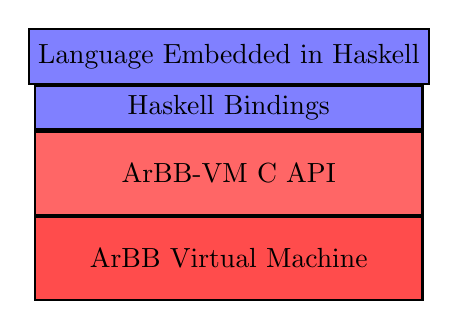
\begin{tikzpicture} 
    
    \node [draw,thick, fill=red!70, minimum width = 14em, 
           minimum height = 3em] 
       (vm)  {ArBB Virtual Machine}; 

    \onslide<2-5>{

    \node [draw,thick, fill=red!60, minimum width = 14em, 
           minimum height = 3em, above= 0pt of vm] 
       (capi) {ArBB-VM C API}; 
    }

    \onslide<3>{

    \node [draw,thick, fill=red!50, minimum width = 14em, 
           minimum height = 3em, above= 0pt of capi] 
       (cpp) {Language Embedded in C++}; 
    }
    
    \onslide<4-5> { 
      \node [draw,thick, fill=blue!50, minimum width = 14em, 
        minimum height = 1em, above= 0pt of capi] 
        (bindings) {Haskell Bindings}; 
    }
    \onslide<5> { 
      \node [draw,thick, fill=blue!50, minimum width = 14em, 
        minimum height = 2em, above= 0pt of bindings] 
        (embarbb) {Language Embedded in Haskell}; 
    }

    
    
  \end{tikzpicture}
  \end{center} 

\end{frame} 

% -------------------------------------------------------------------------
%
% -------------------------------------------------------------------------

\begin{frame}[fragile]{EmbArBB Code} 

\begin{block}{}
\Fontvi
\begin{verbatim}
matVec :: Exp (DVector Dim2 Float) 
        -> Exp (DVector Dim1 Float) 
        -> Exp (DVector Dim1 Float) 
matVec m v = addReduce rows 
           $ m * (repeatRow (getNRows m) v)
\end{verbatim} 
\end{block} 

\end{frame} 

\begin{frame}[fragile]{EmbArBB Code} 

\begin{block}{}
\Fontvi
\begin{verbatim}
main =  
  withArBB $ 
  do 
     f <- capture matVec  
     let m1 = V.fromList [2,0,0,0,
                          0,2,0,0,
                          0,0,2,0,
                          0,0,0,2]
         v1 = V.fromList [1,2,3,4] 
     
     m <- copyIn $ mkDVector m1 (Z:.4:.4) 
     v <- copyIn $ mkDVector v1 (Z:.4) 

     r1 <- new (Z:.4) 0 

     execute f (m :- v)  r1
              
     r <- copyOut r1
              
     liftIO$ putStrLn$ show r
\end{verbatim} 
\end{block} 

\end{frame} 



\begin{frame}{EmbArBB: Performance} 

 \begin{minipage}{.48\linewidth}
 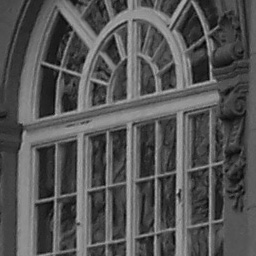
\includegraphics[width=\linewidth]{window.jpg}
 \end{minipage} %
 \begin{minipage}{.48\linewidth}
 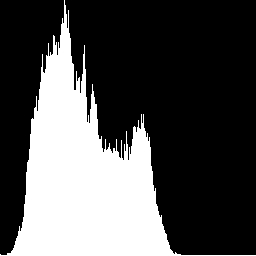
\includegraphics[width=\linewidth]{histogram.jpg}
 \end{minipage}

\end{frame} 

\begin{frame}{EmbArBB: Performance} 

 \begin{minipage}{.48\linewidth}
 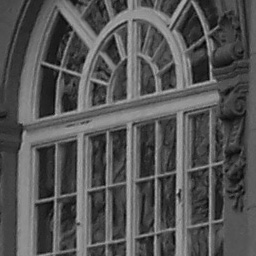
\includegraphics[width=\linewidth]{window.jpg}
 \end{minipage} %
 \begin{minipage}{.48\linewidth}
 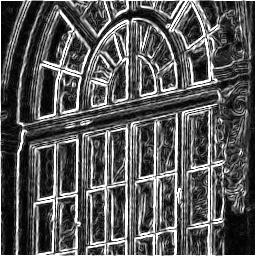
\includegraphics[width=\linewidth]{sobout.jpg}
 \end{minipage}

\end{frame} 

\begin{frame}{EmbArBB: Performance} 

 \begin{minipage}{.48\linewidth}
 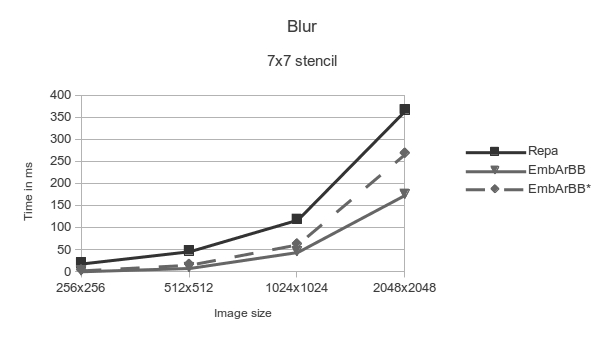
\includegraphics[width=\linewidth]{blurchart.jpg}
 \end{minipage} %
 \begin{minipage}{.48\linewidth}
 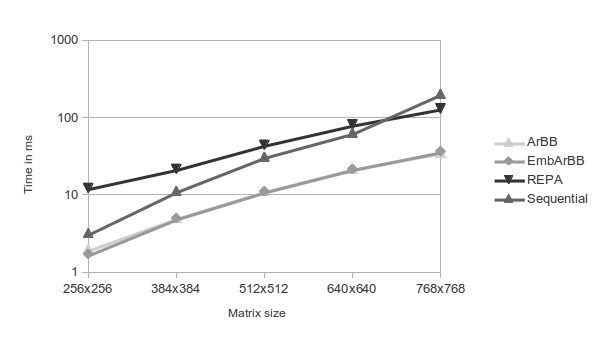
\includegraphics[width=\linewidth]{mmchart1.jpg}
 \end{minipage}

\end{frame} 


\section{Related Work} 

\begin{frame}{Related Work} 
\begin{center}
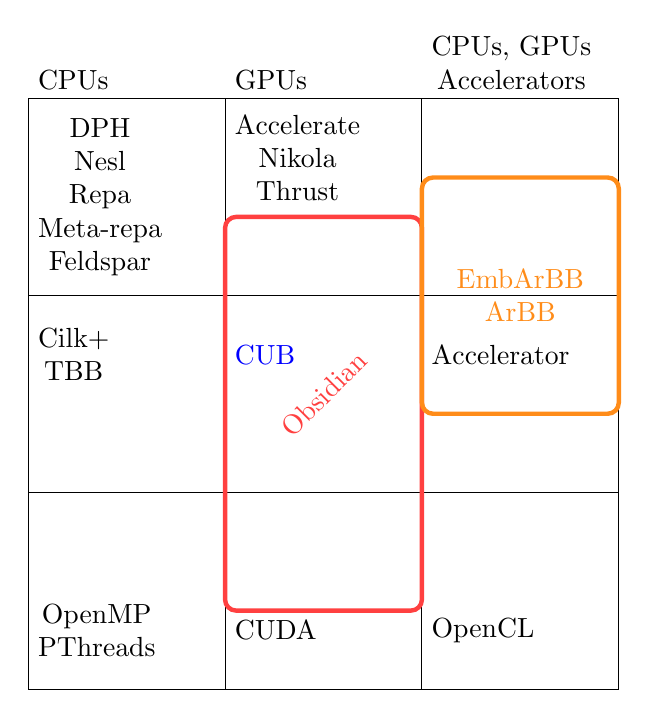
\begin{tikzpicture}[align=center, scale=2.5]
% \draw[help lines] (0,0) grid (3,3);


%\draw[->] (-0.5,0) -- (-0.5,3) node[anchor=east] {Abstraction level};

\draw (0,3) node[anchor=south west] {CPUs};
\draw (1,3) node[anchor=south west] {GPUs};
%\draw (2,3) node[anchor=south west] {Accelerator};
\draw (2,3) node[anchor=south west] {CPUs, GPUs\\ Accelerators};

\node[anchor=west] (acc) at (1,2.7) {Accelerate\\Nikola\\Thrust};
\node[anchor=west,blue!100] (cub) at (1,1.7) {CUB};
\node[anchor=west] (repa) at (0,2.5) {DPH\\Nesl\\Repa\\Meta-repa\\Feldspar};
\node[anchor=west] (mixed) at (0,1.7) {Cilk+\\ TBB};
\node[anchor=west] (accelerator) at (2,1.7) {Accelerator};

\node[anchor=west] (cuda) at (1,0.3) {CUDA};
\node[anchor=west] (opencl) at (2,0.3) {OpenCL};

\node[anchor=west] (OpenMP) at (0,0.3) {OpenMP\\PThreads};

\foreach \x in {0,...,2} { 
  \foreach \y in {0,...,2} { 
    \draw (\x,\y) rectangle (\x+1,\y+1);
  }
}

\draw[red!75,rounded corners,ultra thick] (1,0.4) rectangle (2,2.4);
\node[red!75,rotate=45,thick] (obs) at (1.5,1.5) {Obsidian};

\draw[orange!90,rounded corners,ultra thick] (2,1.4) rectangle (3,2.6);
\node[orange!90,thick] (arbb) at (2.5,2) {EmbArBB\\ArBB};


\end{tikzpicture}
\end{center}
\end{frame} 


% -------------------------------------------------------------------------
%
% -------------------------------------------------------------------------
\begin{frame}{Related Work: Accelerate} 
\begin{center} 

\begin{tikzpicture}[remember picture,
      start chain=going right,
      outer/.style={on chain, node distance=1em},
      every join/.style={->,thick},
      inner/.style={circle,draw=blue!50,fill=blue!20,thick,inner sep=1pt},
    ]

  \node [outer,draw,very thick, rounded corners,join] {Inputs}; 
  \node [outer,draw=gray!50,very thick, rounded corners,minimum height=5.5em,minimum width = 6.5em,join] (apa) {
    \begin{tikzpicture} 
      \node [draw=black!100,inner,minimum size=1pt] (k1) {k1};
      \node [draw=black!100,inner,minimum size=1pt, below= 1em of k1] (k2) {k2};
      \node [draw=black!100,inner,minimum size=1pt, right= 1em of k1] (k3) {k3}; 
    \end{tikzpicture}

  }; 
  \node [outer,draw,very thick, rounded corners,join] {Outputs}; 
  

  \draw (k1) -- (k3)
        (k2) -- (k3)
        (apa.west) -- (k1.west)
        (apa.west) -- (k2.west) 
        (k3.east) -- (apa.east); 
  

\end{tikzpicture} 

\onslide<2>{ 
  \begin{tikzpicture}[overlay, remember picture]
    \node [draw,fill=gray!50,thick, rounded corners] at (-3,-1) {
      \begin{minipage}{5cm} 
        Accelerate: 
         \begin{itemize}  
         \item ks are chosen from a set of primitives
           \begin{itemize}
             \item Map
             \item Fold
             \item Permute
             \item .. 
           \end {itemize} 
         \item Coordination / Composition
         \end{itemize}
      \end{minipage} 
      
    };
  \end{tikzpicture} 
} 
\end{center}
\end{frame} 

% ---------------------------------------------------------------------------
%
% ---------------------------------------------------------------------------

\begin{frame}{Related Work: Accelerate}
\begin{center} 

\begin{tikzpicture}[remember picture,
      start chain=going right,
      outer/.style={on chain, node distance=1em},
      every join/.style={->,thick},
      inner/.style={circle,draw=blue!50,fill=blue!20,thick,inner sep=1pt},
    ]

  \node [outer,draw,very thick, rounded corners,join] {Inputs}; 
  \node [outer,draw=gray!50,very thick, rounded corners,minimum height=5.5em,minimum width = 6.5em,join] (apa) {
    \begin{tikzpicture} 
      \node [draw=black!100,inner,minimum size=1pt] (k1) {k1};
      \node [draw=black!100,inner,minimum size=1pt, below= 1em of k1] (k2) {k2};
      \node [draw=black!100,inner,minimum size=1pt, right= 1em of k1] (k3) {k3}; 
    \end{tikzpicture}

  }; 
  \node [outer,draw,very thick, rounded corners,join] {Outputs}; 
  

  \draw (k1) -- (k3)
        (k2) -- (k3)
        (apa.west) -- (k1.west)
        (apa.west) -- (k2.west) 
        (k3.east) -- (apa.east); 
  

\end{tikzpicture} 

  \begin{tikzpicture}[overlay, remember picture]
    
   \node [draw, circle,very thick, minimum size=2em] (magni) at (-0.58,2.05) {};
    
   \node [draw, very thick] (test) at (-1,0) {
     \begin{tikzpicture}
       \node [draw, fill=red!50] (b0) {Block 0};
       \node [draw, fill=red!50, below=0pt of b0] (b1) {Block 1};
       \node [below=0pt of b1] (bdots) {\huge \ldots};
       \node [draw, fill=red!50, below=0pt of bdots] (bN) {Block N};
       

     \end{tikzpicture} 

   };

   \draw [very thick] (magni) -- (test);
  \end{tikzpicture}

  \begin{tikzpicture}[overlay, remember picture]
    \node [draw,fill=gray!50,thick, rounded corners] at (3,-1) {
      \begin{minipage}{5cm} 
        Obsidian: 
         \begin{itemize}  
         \item Program what the ks do
         \end{itemize}
      \end{minipage} 
      
    };
  \end{tikzpicture} 



\end{center}
\end{frame} 





% -------------------------------------------------------------------------
%
% -------------------------------------------------------------------------
\section{Future Work}
\begin{frame}{Future Work}
Obsidian:
  \begin{itemize} 
    \item Warp level capabilities
    \item Optimisations? 
    \item Smarter compiler? 
    \item Kernel Coordination (full applications) 
  \end{itemize} 
EmbArBB: 
  \begin{itemize} 
    \item ArBB doesn't exist anymore 
      \begin{itemize} 
        \item Retarget EmbArBB to another code generator
        \item Hope someone revives ArBB
      \end{itemize} 
      
  \end{itemize} 
  
\end{frame} 


\begin{frame}{Extra} 

Extra slides

\end{frame}

\begin{frame}[fragile]{Obsidian: Execute Generated Code}
  
  \begin{block}{}
    \Fontvi
\begin{verbatim}
perform =
  withCUDA $
  do
    kern <- capture 256 (incK . splitUp 256) 

    useVector (V.fromList [0..255 :: Int32]) $ \i ->
      useVector (V.fromList (P.replicate 256 (0 :: Int32))) $ \ o ->
      do
        o <== (1,kern) <> i 
        r <- peekCUDAVector o
        lift $ putStrLn $ show r     
\end{verbatim} 
  \end{block}
\end{frame} 


\begin{frame}{Data-Parallelism: Increment}
\begin{center} 
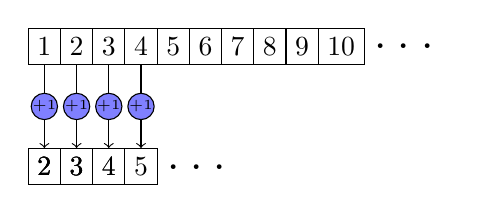
\begin{tikzpicture}[
      start chain=1 going right,start chain=2 going below,node distance=-0.15mm
    ]


  \foreach \x in {1,2,...,10} {
    \node (\x) [draw, on chain=1] {\x};
  }
  \node [on chain=1] {\huge \ldots};
  
  

  \onslide<2>{
    \node [draw, below=3em of 1] (r1) {2};
    % \draw [->] (1) -- (r1);
    \addone{1}{r1}
    }

  \onslide<3>{
    \node [draw, below=3em of 1] (r1) {2};
    \node [draw, below=3em of 2] (r2) {3};
    %\draw [->] (2) -- (r2);
    \addone{2}{r2}
    }


  \onslide<4>{
    \node [draw, below=3em of 1] (r1) {2};
    \node [draw, below=3em of 2] (r2) {3};
    \node [draw, below=3em of 3] (r3) {4};
    %\draw [->] (3) -- (r3);
    \addone{3}{r3}
    }

  \onslide<5>{
    \node [draw, below=3em of 1] (r1) {2};
    \node [draw, below=3em of 2] (r2) {3};
    \node [draw, below=3em of 3] (r3) {4};
    \node [draw, below=3em of 4] (r4) {5};
    %\draw [->] (4) -- (r4);
    \addone{4}{r4}
    \node [right=-0.15mm of r4] {\huge \ldots};
    }
  
\end{tikzpicture} 
\end{center}
\end{frame}

% -------------------------------------------------------------------------
%
% -------------------------------------------------------------------------
\begin{frame}{Data-Parallelism: Increment in Parallel}
\begin{center} 
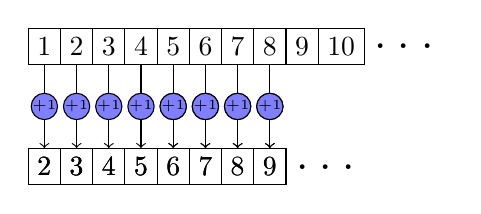
\begin{tikzpicture}[
      start chain=1 going right,start chain=2 going below,node distance=-0.15mm
    ]


  \foreach \x in {1,2,...,10} {
    \node (\x) [draw, on chain=1] {\x};
  }
  \node [on chain=1] {\huge \ldots};
  
  

  \onslide<2>{
    \node [draw, below=3em of 1] (r1) {2};
    \node [draw, below=3em of 2] (r2) {3};
    \node [draw, below=3em of 3] (r3) {4};
    \node [draw, below=3em of 4] (r4) {5};

    \addone{1}{r1}
    \addone{2}{r2}
    \addone{3}{r3}
    \addone{4}{r4}
    }

  \onslide<3>{
    \node [draw, below=3em of 1] (r1) {2};
    \node [draw, below=3em of 2] (r2) {3};
    \node [draw, below=3em of 3] (r3) {4};
    \node [draw, below=3em of 4] (r4) {5};
    \node [draw, below=3em of 5] (r5) {6};
    \node [draw, below=3em of 6] (r6) {7};
    \node [draw, below=3em of 7] (r7) {8};
    \node [draw, below=3em of 8] (r8) {9};

    \addone{5}{r5}
    \addone{6}{r6}
    \addone{7}{r7}
    \addone{8}{r8}
    }

  \onslide<3>{
    \node [draw, below=3em of 1] (r1) {2};
    \node [draw, below=3em of 2] (r2) {3};
    \node [draw, below=3em of 3] (r3) {4};
    \node [draw, below=3em of 4] (r4) {5};
    \node [draw, below=3em of 5] (r5) {6};
    \node [draw, below=3em of 6] (r6) {7};
    \node [draw, below=3em of 7] (r7) {8};
    \node [draw, below=3em of 8] (r8) {9};

    \addone{5}{r5}
    \addone{6}{r6}
    \addone{7}{r7}
    \addone{8}{r8}

    \node [right=-0.15mm of r8] {\huge \ldots};
    }

\end{tikzpicture} 

\end{center}
\end{frame}


% -------------------------------------------------------------------------
%
% -------------------------------------------------------------------------
\begin{frame}[fragile]{GPU Programming: CUDA Example}

\begin{block}{}
\begin{tiny}
\begin{verbatim} 
main(void) {
  
  int32_t h_a[32], h_r[32]; 
  int32_t *d_a, *d_r;
  
  for (int i = 0; i < 32; ++i) 
    h_a[i] = i;

  cudaMalloc((void**)&d_a,32*sizeof(int32_t));
  cudaMalloc((void**)&d_r,32*sizeof(int32_t));

  cudaMemcpy(d_a,h_a,32*sizeof(int32_t),
                     cudaMemcpyHostToDevice);
  
  inc<<<1,32,0>>>(d_a,d_r); 

  cudaMemcpy(h_r,d_r,32*sizeof(int32_t),
                     cudaMemcpyDeviceToHost);

  for (int i = 0; i < 32; ++i) 
    printf("%d ",h_r[i]);
}
\end{verbatim}
\end{tiny}
\end{block} 
\end{frame} 


\begin{frame}{Embedded Languages} 

  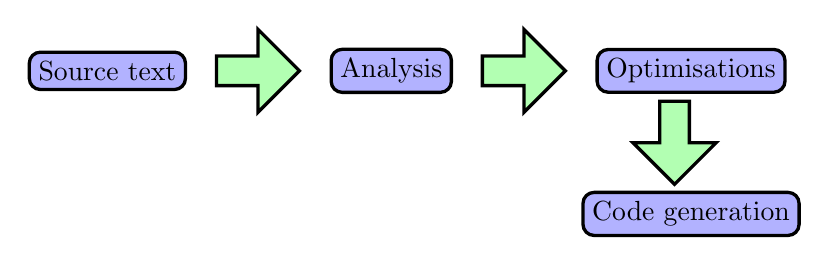
\begin{tikzpicture} 
    
    %\onslide<1-5>{
    \node [draw, fill=blue!30, very thick, rounded corners] 
      (source) {Source text}; 
    %}
    \onslide<2-5>{ 
      \node [draw, fill=green!30, 
             very thick, 
             minimum size = 3em,
             single arrow, 
             right=1em of source] (a1) {};

      \node [draw, fill=blue!30, 
             very thick, rounded corners, 
             right=1em of a1] (analysis) {Analysis};
    }
    \onslide<4-5>{
      
      \node [draw, fill=green!30, 
             very thick, 
             minimum size = 3em,
             single arrow, 
             right=1em of analysis] (a1) {};
      
      \node [draw, fill=blue!30, 
             very thick, rounded corners, 
             right=1em of a1] (opt) {Optimisations};
      
    }
    \onslide<5>{
       \node [draw, fill=green!30, 
             very thick, 
             minimum size = 3em,
             single arrow, rotate=270, 
             below=1.5em of opt] (a1) {};
      
      \node [draw, fill=blue!30, 
             very thick, rounded corners, 
             below=3.5em of opt] (codegen) {Code generation}; 
    }

  \end{tikzpicture}

  \onslide<3>{ 
    \begin{tikzpicture}[overlay, remember picture] 
      \node [draw] at (5,0) (details1) {
         \begin{tikzpicture} 
           \node (text1) {``2 * a + 1''}; 
           \node [draw, thick, 
                  single arrow, 
                  minimum size=2em, right=1em of text1] 
           (localarr) {};
           \node [draw, circle,thick,inner sep=1pt] (pnode) at (4,0.7) {$+$};
           \node [draw, circle,thick,inner sep=2pt, below left=1em and 1em of pnode](mnode)  {$*$}; 
           \draw (pnode) -- (mnode);

           \node [below left=1em and 1em of mnode] (two) {$2$};
           \node [below right=1em and 1em of mnode] (anode) {$a$}; 
           \node [below right=1em and 1em of pnode] (onenode) {$1$};

           \draw (mnode) -- (two) 
                 (mnode) -- (anode) 
                 (pnode) -- (onenode); 
           
         \end{tikzpicture} 
        };
    \end{tikzpicture}
  }

%       + 
%   *       1 
% 2   a 

\end{frame} 

% -------------------------------------------------------------------------
%
% -------------------------------------------------------------------------
\begin{frame}{Embedded Languages} 

  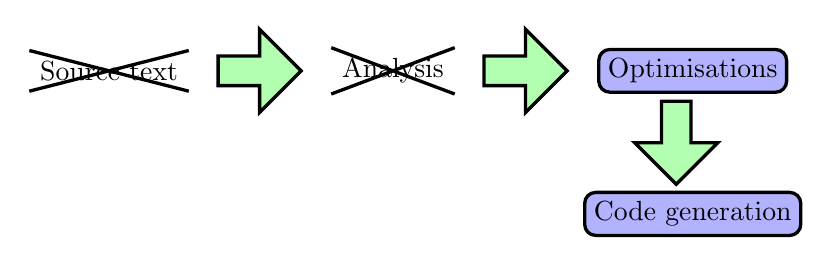
\begin{tikzpicture} 
    
    \node [draw, very thick, cross out] 
      (source) {Source text}; 
    
    \node [draw, fill=green!30, 
           very thick, 
           minimum size = 3em,
           single arrow, 
           right=1em of source] (a1) {};

    \node [draw, cross out, 
           very thick,
           right=1em of a1] (analysis) {Analysis};

    
    \node [draw, fill=green!30, 
           very thick, 
           minimum size = 3em,
           single arrow, 
           right=1em of analysis] (a1) {};
      
    \node [draw, fill=blue!30, 
           very thick, rounded corners,
           right=1em of a1] (opt) {Optimisations};
      
    \node [draw, fill=green!30, 
           very thick, 
           minimum size = 3em,
           single arrow, rotate=270, 
           below=1.5em of opt] (a1) {};
      
    \node [draw, fill=blue!30, 
           very thick, rounded corners, 
           below=3.5em of opt] (codegen) {Code generation}; 
    
  \end{tikzpicture}

  \begin{tikzpicture}[overlay, remember picture]     
    \node [draw, fill=blue!30, 
           very thick, rounded corners] at (8.55,4.75) (lib) {Library};
    \node [draw, fill=green!30, 
           very thick, 
           minimum size = 3em,
           single arrow, rotate=270, 
           below right=0.8em and -1em of lib] (a1) {};
    
  \end{tikzpicture} 

\end{frame} 

%% \begin{frame}{GPU Programming: NVIDIA CUDA}
%% \begin{center} 

%% \begin{tikzpicture}[
%%       start chain=1 going right,start chain=2 going below,node distance=1em,
%%       every join/.style={->,thick},
%%     ]

%%   \node [draw,very thick, rounded corners, on chain=1,join] {Inputs}; 
%%   \node [draw,very thick, rounded corners, on chain=1,minimum height=5.5em,minimum width = 6.5em,join] {\huge ?}; 
%%   \node [draw,very thick, rounded corners, on chain=1,join] {Outputs}; 
  

%% \end{tikzpicture} 
%% \end{center}

%% \end{frame}

%% % -------------------------------------------------------------------------
%% %
%% % -------------------------------------------------------------------------

%% \begin{frame}{GPU Programming: NVIDIA CUDA}
%% \begin{center} 

%% \begin{tikzpicture}[remember picture,
%%       start chain=going right,
%%       outer/.style={on chain, node distance=1em},
%%       every join/.style={->,thick},
%%       inner/.style={circle,draw=blue!50,fill=blue!20,thick,inner sep=1pt},
%%     ]

%%   \node [outer,draw,very thick, rounded corners,join] {Inputs}; 
%%   \node [outer,draw=gray!50,very thick, rounded corners,minimum height=5.5em,minimum width = 6.5em,join] (apa) {
%%     \begin{tikzpicture} 
%%       \node [draw=black!100,inner,minimum size=1pt] (k1) {k1};
%%       \node [draw=black!100,inner,minimum size=1pt, below= 1em of k1] (k2) {k2};
%%       \node [draw=black!100,inner,minimum size=1pt, right= 1em of k1] (k3) {k3}; 
%%     \end{tikzpicture}

%%   }; 
%%   \node [outer,draw,very thick, rounded corners,join] {Outputs}; 

%%   \draw (k1) -- (k3)
%%         (k2) -- (k3)
%%         (apa.west) -- (k1.west)
%%         (apa.west) -- (k2.west) 
%%         (k3.east) -- (apa.east); 
  

  

%% \end{tikzpicture} 

%% \onslide<2-5>{
%%   \begin{tikzpicture}[overlay, remember picture]
    
%%    \node [draw, circle,very thick, minimum size=2em] (magni) at (-0.58,2.05) {};
    
%%    \node [draw, very thick] (test) at (-1,0) {
%%      \begin{tikzpicture}
%%        \node [draw, fill=red!50] (b0) {Block 0};
%%        \node [draw, fill=red!50, below=0pt of b0] (b1) {Block 1};
%%        \node [below=0pt of b1] (bdots) {\huge \ldots};
%%        \node [draw, fill=red!50, below=0pt of bdots] (bN) {Block N};
       

%%      \end{tikzpicture} 

%%    };

%%    \draw [very thick] (magni) -- (test);
%%   \end{tikzpicture}
%% }

%% \onslide<3>{ 
%%   \begin{tikzpicture}[overlay, remember picture]
%%     \node [fill=gray!50] at (2,0) {
%%       \begin{minipage}{3.5cm}
%%       Block:
%%       \begin{small}
%%       \begin{itemize}
%%         \item Many threads
%%         \item Shared memory
%%         \item Synchronize
%%         \item Same program 
%%         \item Different data
%%       \end{itemize}
%%       \end{small}
%%       \end{minipage}
%%     };
%%   \end{tikzpicture}
%% }

%% \onslide<4>{ 
%%   \begin{tikzpicture}[overlay, remember picture]
%%     \node [fill=gray!50] at (2,0) {
%%       \begin{minipage}{3.5cm}
%%       Warp:
%%       \begin{small}
%%       \begin{itemize}
%%         \item 32 threads
%%         \item Scheduled unit
%%         \item Lockstep
%%       \end{itemize}
%%       \end{small}
%%       \end{minipage}
%%     };
%%   \end{tikzpicture}
%% }

%% \onslide<5>{ 
%%   \begin{tikzpicture}[overlay, remember picture]
%%     \node [fill=gray!50] at (2,0) {
%%       \begin{minipage}{3.5cm}
%%       Grid:
%%       \begin{small}
%%       \begin{itemize}
%%         \item Collection of all blocks
%%       \end{itemize}
%%       \end{small}
%%       \end{minipage}
%%     };
%%   \end{tikzpicture}
%% }



%% \end{center}

%% \end{frame}


%\begin{frame}{}
%  End
%\end{frame} 


\end{document} 
